\documentclass{standalone}
\usepackage{tikz}
\usetikzlibrary{arrows.meta, bending, positioning, intersections, backgrounds}

\begin{document}
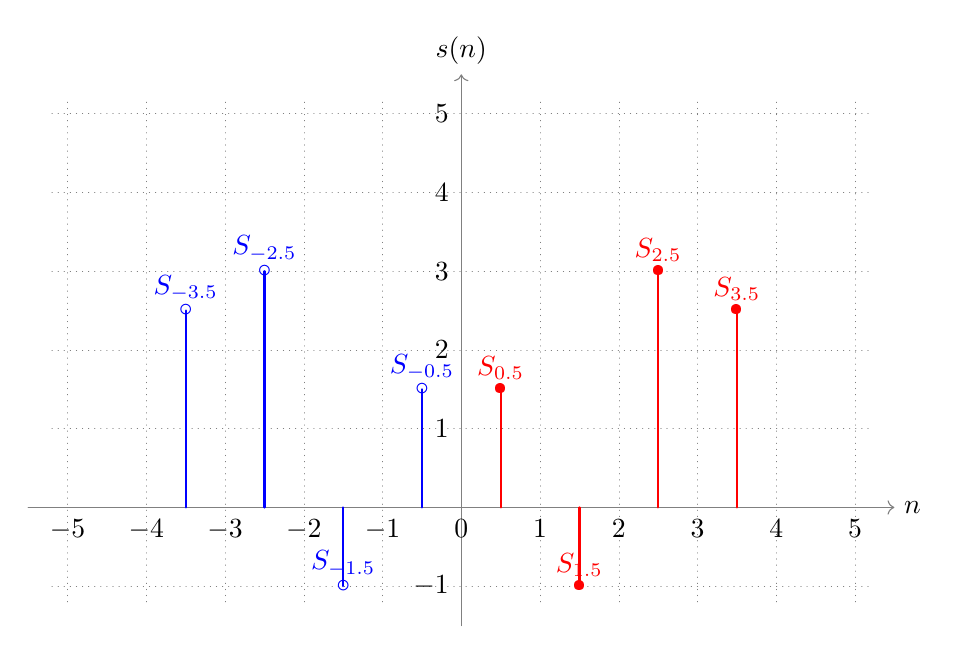
\begin{tikzpicture}
% Style
[
    scale=1, line cap=round, axes/.style=,
    important line/.style={very thick},
    information text/.style={rounded corners,fill=red!10,inner sep=1ex}
]

% Define: Params
\newcommand{\orioffset}{+0.5} %ori_offset
\newcommand{\dstoffset}{-0.5} %dst_offset

%================================== Prepare ==================================
\newcommand{\drawhistogram}[5]{
    % Draw: lollipop
    \node[#3] at (#1#5,#2) {#4};
    \node[#3, above] at (#1#5,#2) {$S_{\fpeval{#1+#5}}$};
    \draw[#3, thick] (#1#5, 0.0)--(#1#5,#2);
}

%=================================== Start ===================================
{
    % Define: Axis
    \draw [help lines, dotted, gray] (-5.2,-1.2) grid (5.2,5.2);
    \begin{scope}[axes]
        \draw[->, thin, draw=gray] (-5.5,0)--(5.5,0) node [right] {$n$} coordinate(x axis);
        \draw[->, thin, draw=gray] (0,-1.5)--(0,5.5) node [above] {$s(n)$} coordinate(y axis);
        \foreach \x in {-5, ..., 5} {
            \draw (\x, -1pt) node[below] {$\x$};
        }
        \foreach \y in {-1, ..., -1} {
            \draw (-1pt, \y) node[left] {$\y$};
        }
        \foreach \y in {1, ..., 5} {
            \draw (-1pt, \y) node[left] {$\y$};
        }
    \end{scope}

    % Draw: Samples
    \foreach \x / \y in {0/1.5, 1/-1, 2/3, 3/2.5} {
        \drawhistogram{\x}{\y}{red}{\textbullet}{\orioffset}; 
    }

    % Draw: Supplies
    \foreach \x / \y in {0/1.5, -1/-1, -2/3, -3/2.5} {
        \drawhistogram{\x}{\y}{blue}{$\circ$}{\dstoffset}; 
    }
}
%==================================== END ====================================

\end{tikzpicture}
\end{document}